\section*{\textbf{\underline{Abstract}}}
Plant-animal transport mutualisms, such as seed dispersal and pollination, represent a diverse suite of interactions that impact the function and dynamics of many ecological communities. Network representations of these interactions exhibit a wide range of structural properties (e.g. nestedness, modularity) that ultimately mediate emergent properties of ecological relevance (e.g. stability, resilience, robustness to secondary extinction). Understanding how these structural properties are affected by anthropogenic forcing and how they scale up to shape emergent properties is vital for predicting and conserving mutualistic networks in the face of global change. Here, I review the current state of knowledge on how three major classes of anthropogenic impact: shifts in global climate, land use intensification, and human-mediated invasion, affect the structural properties of plant-animal transport mutualism networks. In particular, I synthesize emerging patterns and persistent knowledge gaps in how these drivers alter network structure across systems and scales. Finally, I highlight a series of open questions in the field, the answers to which may help elucidate how these structural shifts scale up to changes in community dynamics, and ultimately improve our ability to predict and conserve mutualistic systems.

\section*{\textbf{\underline{Introduction}}}
\paragraph*{Mutualisms are important to the function of ecosystems}\mbox{}\\ 
The term "mutualism" covers a broad suite of species interactions, many of which are collectively vital to the function of many ecosystems as we currently know them \parencite{boucher1982ecology}, and iconic organismal features such as flowers or fruits are living homages to the mutualisms that they support \parencite{weiblen2015evolutionary}. The flow of resources facilitated by these and other mutualistic interactions can serve key ecological functions, and ultimately provide significant ecosystem services to human communities across the planet. Globally, pollinators may provide as much as \$400 billion annually in agricultural pollination services alone as of 2020 \parencite{porto2020pollination}, and are relied upon by 85\% of extant plant species across the globe \parencite{ollerton2011many}.
    

\paragraph{}
Due to their outsized impact on ecosystem function and services, understanding how mutualistic interactions change in response to perturbation is of great interest. These influential interactions do not happen in a vacuum, and taking a network approach to studying mutualisms can better allow us to understand how mutualisms as a whole affect the structure, function, and resultant services provided by an ecosystem. N	etwork approaches allow us to more clearly understand how perturbations propagate through a system, and have been used to study consumer-resource interactions \parencite{rooney2012integrating}, nutrient cycles, \parencite{christian1996nitrogen}, host-parasite interactions, \parencite{dallas2015co}, and mutualistic interactions \parencite{vanbergen2017network, rohr2014structural}. Together, these approaches have enhanced the ability to predict how diverse communities may respond to environmental change. In order to understand how communities of interacting species may change in the face of growing anthropogenic forcing, it is vital to understand how human-induced changes tend to affect the structure and function of mutualistic networks. 

%There have been massive changes in mutualistic networks
\paragraph*{}
Global ecosystems are subject to anthropogenically driven changes at increasing rates, and as a result, so are the mutualistic interaction networks that occur within them. Structural changes in mutualistic networks can be driven by a diverse set of drivers, including shifting climates, urbanization and land use changes, and invasion of non-native species. Here, I aim to characterize the current state of understanding about the ways these diverse drivers affect the structural properties of two major classes of plant-animal transportation mutualisms \parencite{bronsteinmutualism1}: seed dispersal and pollination networks, as well as how we can leverage our knowledge of these patterns to better understand, predict, and conserve these critical natural systems. 


% TD: you use 'we' 30 times. It's a bit informal to use this, but I also don't want to tell you to use the passive voice too much. Maybe change some of them, because I'm already picking up on it at this point and I think a reviewer will too. 

\paragraph*{Emergent Properties of Mutualist Networks}\mbox{}\\ 
The structure of relationships within mutualistic systems can generate dynamic system-level behavior, including several emergent properties useful for understanding how mutualistic systems may respond to perturbation (Figure \ref{fig:ConceptDraft}). These include properties describing how mutualistic networks behave around equilibrial states, a number of which can be estimated through eigenanalysis of the Jacobian matrix representing mutualistic communities at equilibrium. Both local stability (the tendency of the system to dampen small perturbations from equilibrium) \parencite{valdovinos2019mutualistic, okuyama2008network}, as well as resilience (here, the speed at which the system returns to equilibrium after perturbation) \parencite{thebault2010stability, suweis2013emergence}, are important for predicting how mutualistic networks respond to anthropogenic change. Other properties include the size of the feasibility domain, the range of parameter values that permits non-zero equilibrium abundances for all species in a community \parencite{saavedra2016nested, grilli2017feasibility, wang2023interspecific}. This property, sometimes referred to as structural stability, defines the safe operational space within which all species can persist \parencite{bascompte2022resilience}. Given an existing network structure, the extent to which disturbances spread widely or remain confined to local subsets of species \parencite{martins2024propagation, suweis2015effect} is yet another emergent feature of interest in the context of anthropogenic change, and is closely related to the structural property of modularity. 


\paragraph{}
These metrics collectively provide important insights into how existing network structure may mediate the impact of perturbation, but we are also interested in how networks may be sensitive to changes to their existing structure. By definition, mutualistic partners improve one another's fitness; if the magnitude of benefit scales in some way with population size \parencite{valdovinos2019mutualistic}, positive feedbacks between partnered populations or threshold responses \parencite{hale2021ecological} may occur. Disrupting these positive feedbacks of networks can facilitate critical transitions, and structural properties of networks can be important for determining behavior at the critical boundary or determining how robust a network is to loss of certain nodes or links \parencite{van2021facultative}. For example, simulated plant-pollinator networks with greater connectance are more likely to undergo large critical transitions as extinctions occur, undergoing larger community-level breakdowns instead of many small breakdowns \parencite{lever2014sudden}. Positive feedbacks may also induce hysteretic effects crossing the critical transition boundary; that is community assembly and disassembly processes may often be non-symmetric in mutualistic systems, with the outcome depending on precursor system states \parencite{cai2020mutualistic}. Understanding how these processes occur and are influenced by network structural properties is vital for both prediction and conservation of mutualistic systems.


\paragraph*{The Importance of Structural Properties}\mbox{}\\ 
%Structural features affect emergent ones
Many of these aforementioned emergent properties of interest (stability, resilience, hysteresis, etc.) are heavily impacted by network structural properties \parencite{landi2018complexity}. A significant body of existing literature has been devoted to interrogating relationships between the structural properties and emergent properties of species interaction networks, though at times with counterintuitive results. For example, network modularity (the property of having more connections within smaller subunits of a network than between them) tends to reduce the propagation of direct or indirect perturbations through a mutualistic system \parencite{thebault2010stability, okuyama2008network}. Invasion by non-native generalist species increases connectance and decreases modularity of some networks, potentially leading to broader or faster propagation of disturbances in the face of a changing environment \parencite{fricke2020accelerating, vollstadt2022plant, martins2024propagation}.  Because of their important and often complex effects on emergent properties, understanding how network structural properties tend to change in response to anthropogenic forcing is vital for prediction and management of mutualistic systems. 

%How structure -> Emergent is complicated
\paragraph*{} 
Structural properties often have nuanced effects on multiple emergent properties, making it important to identify which emergent properties are most relevant in a given context. For example, one widely observed property of mutualistic networks is nestedness, in which specialist species with few interaction partners tend to interact with generalist species that have many partners, effectively embedding specialist interactions within a broader, generalist core \parencite{bascompte2003nested, bascompte2006asymmetric, thebault2010stability}. As nestedness increases, the overall robustness of the system to species loss may increase due to functional redundancy, while simultaneously making the final breakdown of the system more dramatic (increasing magnitude of critical transitions) \parencite{bascompte2022resilience}. The nestedness of strong interactions tends to increase the size of a mutualistic system's feasibility domain \parencite{saavedra2016nested}, yet decrease its stability at equilibrium \parencite{allesina2012stability}. However, even if more nested mutualistic networks are less stable, they may lead to higher overall community abundance, an effect stronger in systems characterized by abundant but weak mutualisms \parencite{suweis2013emergence}. Robert May first pointed out in 1973 the ``paradox of complex interactions", where, under a Lotka-Volterra style modeling framework, larger species assemblages with many strong and randomly assigned species interactions lead to correspondingly smaller feasible domains of community stability \parencite{may1973stability}, a pattern that tends to be even more pronounced in mutualistic systems \parencite{allesina2012stability, saavedra2016nested}.  In reality, however, interactions are not randomly assigned within a community, and empirically observed suites of mutualistic interactions often tend to favor stability in practice, though to varying degrees \parencite{thebault2010stability, grilli2017feasibility}. How structural properties translate into emergent ones may be further complicated by plasticity in species interaction preferences \parencite{corro2021annual} or the degree of nodes' dependence on mutualisms \parencite{van2021facultative}. Valdovinos et al. (2016) found that accounting for potential adaptive foraging behaviors reversed the effects of nestedness and connectance on species persistence times \parencite{valdovinos2016niche}. In general, the relationship between structural and emergent properties is complicated and can lead to counterintuitive results \parencite{landi2018complexity}.

\paragraph*{} %How do structural features arise? 
The mechanisms under which emergent properties arise in networks across a landscape still warrant further investigation, especially in the context of mutualistic systems. In food webs, Borrelli et al. (2015) found that stabilizing motifs were overrepresented relative to null expectations across a diverse set of 50 networks, potentially indicating the presence of stabilizing processes present across landscape scales \parencite{borrelli2015selection}. This is supported by prior work looking at the constancy of network structural properties across scales in both trophic \parencite{fahimipour2014dynamics} and host-parasite \parencite{dallas2018compositional} networks, even as individual species turn over across space. The conservation of network properties despite species turnover may indicate that separate assembly mechanisms operate at the level of interaction networks and species assemblages per se \parencite{petanidou2008long, dupont2009spatio, burkle2011future, dehling2020similar, ten2024latitudinal}. One potential set of mechanisms acting on network structure may be non-Darwinian selection processes \parencite{saravia2022ecological}, where more stable networks endure longer through time as less stable networks break down, a potential phenomenon supported by theoretical modeling work \parencite{cai2020mutualistic}. However, one must be cautious in interpreting the prevalence of stabilizing structural properties as evidence for these processes; Saravia et al. (2022) found little difference between realized local networks and random draws from the regional metaweb in trophic networks \parencite{saravia2022ecological}, emphasizing the importance of proper null models in the context of network structure \parencite{maynard2018network, pellissier2018comparing}. Additionally, while different structural measures capture different aspects of network topology, they are seldom independent, a feature well-appreciated in food webs \parencite{vermaat2009major}. Understanding how structural properties covary is another reason null model approaches are important and looking at joint properties may be useful \parencite{fortuna2010nestedness, poisot2014ecological, pellissier2018comparing, dormann2017}. 



%Network properties may also influence individual species fitness components predictably, according to their traits, with even the fitness benefit conveyed by given interactions depending on community structure (ex. Specialists in nested communities had higher closeness centrality. 



\paragraph*{Widely Observed Structural Properties of Mutualistic Networks}\mbox{}\\ 
%Emp Nets are Nested
There are a number of properties pervasive in empirically observed frugivory and floral visitation networks. Empirical networks often exhibit high degrees of interaction nestedness \parencite{fortuna2006habitat, bascompte2006asymmetric}, a product of the asymmetric specialization widely observed in both seed-dispersal \parencite{yohe2025frugivore, schleuning2014loss} and floral visitor networks \parencite{bascompte2003nested}. This feature tends to increase the strength of highly connected nodes, often resulting in long-tailed degree distributions. Especially in pollination systems there may be trade-offs in specialization stemming from this pervasive interaction asymmetry; \parencite{arceo2020plant} found that a plant's degree specialism was positively related to heterospecific pollen delivery, likely due to associations with generalist pollinators \parencite{arceo2020plant}. Nestedness may increase positive indirect interactions within guilds, ultimately increasing the potential diversity of species a community can support \parencite{bascompte2003nested, guimaraes2017indirect}. It also can reduce effective interspecific competition, increasing equilibrial species richness \parencite{bastolla2009architecture}, a pattern potentially observed in empirical networks \parencite{Gonzales2015macroecology}. 

%Emp Nets are Modular
\paragraph*{}
Modularity is another prevalent feature of mutualistic networks, many of which may be separated by functional guilds \parencite{ramos2018modularity} or phylogenetically conserved groups of interaction partners \parencite{Gonzales2015macroecology}. Species with certain traits or within certain taxonomic groups may be more likely to make cross-module connections. Sebasti{\'a}n-Gonz{\'a}lez (2017) found that a small number of highly frugivorous birds and high energy content fruits had higher connectivity both between and within modules \parencite{sebastian2017drivers}. In their study of Peruvian highland pollination networks, Watts et al. (2016) found connector species were likely to be comparatively generalist and taxonomically clustered (\textit{Diptera: Syrphidae} and \textit{Asterales: Asteraceae}). The introduction of a relatively small number of species with higher or lower propensity to establish cross-module connections can fundamentally alter the resultant modularity of a given network \parencite{russo2014patterns}, an idea further explored in the section \textbf{Invasion}.  
%Emp Nets are Sparse? Do I need to talk about this? Ecological networks are generally sparse, a feature that can be a problem for prediction. 
% TD: eh. If the focus was on prediction, I would say sure, but 1 sentence tops should be spent on that, and I'd do it in a section where you talk about how lower-level properties scale to emergent properties (i.e., sparse networks can't really be nested, right?). 


%Emp features may change across space...
\paragraph*{}
Agnostic to changing environments, some evidence shows that network structural properties vary across preexisting environmental or spatial gradients.  In a study of both insect and avian pollination networks across broad latitudinal coverage  Tr{\o}jelsgaard and Olsen (2013) found that modularity was highest at low latitudes whereas nestedness peaked at mid-latitudes \parencite{trojelsgaard2013macroecology}. Across altitudinal gradients, multiple studies have observed an increase in phylogenetic generalism and an associated increase in nestedness and connectance with increasing elevation in plant-pollinator networks \parencite{adedoja2018insect, lara2019beta, classen2020specialization}, though similar evaluations to my knowledge have not been made in frugivory systems. 

%Or climate.
\paragraph*{}
Both the mean and variability of temperature may also play a role in shaping network structural properties; Welti et al. (2015) found that both seed dispersal and floral visitation networks were generally more nested in areas with higher inter-annual temperature variability \parencite{welti2015structure}. Gonz{\'a}lez et al. (2015) found that in mainland plant-hummingbird networks warmer and more stable climates were associated with higher modularity, though these variables had no effect on island networks \parencite{Gonzales2015macroecology}. Both current and past climatic features may have significant effects on network structure \parencite{dalsgaard2013}, further complicating the question of how and at what rate networks may respond to future climatic change. 

\section*{\textbf{\underline{Anthropogenic Change and Mutualistic Network Structure}}}
%Transisition into three drivers sections
While existing environmental conditions have already played a role in shaping mutualistic networks as we know them, human impacts have also drastically altered biotic and abiotic conditions across most of the globe. As natural ecosystems are subject to increasingly severe anthropogenic impacts, so too are the ecological networks that occur within them. Understanding how human-mediated changes affect structural properties and resultant dynamics of mutualistic networks is vital for predicting and conserving species interactions. These changes can occur through several mechanisms, including (1) alterations in community composition, (2) shifts in the probability of interactions occurring, and (3) disruptions to the coevolutionary processes underpinning these networks \parencite{tylianakis2017}. Here, I focus on how three major types of anthropogenic disturbance—climatic shifts, changes in land use, and human-facilitated invasion by non-native species—act through these mechanisms to reshape the structural properties of natural mutualistic networks.
\paragraph*{Climate}\mbox{}\\
Changes in climate can affect mutualistic network structure through a number of mechanisms, including inducing changes in species distributions across time and space, altering species abundances, or altering the physiology of interacting organisms. Many plant-animal mutualisms may only be able to occur during relatively short, yet ecologically important developmental or life history windows. For example, animal pollination can only occur when both the flowering time of the plant and the seasonal activity period of the animal intersect. As climate shifts the timing of these developmental periods, phenological shifts and subsequent mismatches have the potential to occur, altering the strength of mutualistic interactions or even removing them altogether \parencite{zettlemoyer2019phenology, burkle2013plant, teixido2022anthropogenic} . For example, in a forest-prairie floral visitation network Memmott et al. (2007) showed that up to 50\% of floral visitors have reduced overlap between their seasonal activity period and known floral resources over the past century \parencite{memmott2007global}. Link rewiring, in which species form new linkages in response to environmental change, may help alleviate some of the effects of phenological mismatch, but fitness reductions due to reduced phenological overlap with mutualists have been observed empirically \parencite{kudo2019spring, de2023warming}. Corresponding reduction in pollinator fitness have yet to be observed in field systems, though these reductions are likely already occurring in some contexts \parencite{gerard2020global}. These altered interaction probabilities can scale up into altered network structural properties; Encinas-Viso et al. (2012) found in simulated communities that increasing phenological overlap between competitors led to less stable, less nested, and ultimately less speciose communities \parencite{encinas2012phenology}. As climate shifts phenological periods, even if mutualistic interactors remain phenologically coupled, intraguild shifts in species' activity periods (such as overlapping flight or flowering periods) can change competitive interactions with cascading effects through the community \parencite{wang2023interspecific}.
    %Spatial mismatch
    \paragraph*{} 
    Even if mutualistic partners do not become decoupled in time, climate-driven range shifts may also decouple partnerships by reducing spatial overlap. Warming conditions may shift species ranges northward latitudinally or higher in elevation. Differences in features such as generation time and dispersal capacity mean that two mutualistic partners are unlikely to be able to shift their distributions at the same rate. Or, if biotic interactions limit the distributions of some mutualistic species, partners may be unable to shift ranges without commensurate shifts of the distributions of their partners \parencite{warren2014mutualism}. This may be especially salient in the case of seed-dispersal mutualisms, where the ability of plant species to shift their ranges in response to climatic changes may be dependent on their interaction partner \parencite{warren2014mutualism}.

    \paragraph*{}
    While species may shift their distributions or phenology to track preferred environmental conditions, climate change can also alter species abundances, potentially leading to local extirpation. Complete extirpation is not necessary for ecological disruption, however; functional extinction can precede or occur independently of true extirpation when populations become too small to effectively fulfill their roles as mutualists \parencite{costa2018defaunation}. Moreover, mutualistic partners often differ dramatically in their adaptive capacity due to contrasting life histories, such as generation time and population size \parencite{toby2010mutualisms}. For example, the adaptive potential of semelparous insects with annual life cycles differs substantially from that of the long-lived plants they pollinate. Existing work has already shown plant-animal mutualisms are generally weakened by climate change across broad scales \parencite{tylianakis2008global}. Climate-driven extinctions are not necessarily random, and taxonomic or functional biases in abundance changes may have large effects on network properties. Schleuning et al. (2016) found that higher elevation montane mutualism networks were less robust to climate-mediated losses than their lower-elevation counterparts \parencite{schleuning2016ecological}. Limitations to upslope movement have already been shown to reduce population size or extirpate montane species \parencite{freeman2018climate}, potentially putting high elevation mutualistic networks at higher risk of network breakdown. 
    
    %Changes to the phisiology of interactions
    \paragraph*{}
    Changes in environmental conditions may also alter the strength of a given interaction through changes in physiology or interaction preference \parencite{cruz2023mutualisms}, potentially leading to interaction breakdown. Hoover et al. (2012) observed shifts in nectar chemistry as a function of altered pCO$_2$, warming, and nitrogen deposition, which then had downstream effects on experimental pollinator preference and longevity \parencite{hoover2012warming}. Similar changes in pollen quality may also affect nutritional rewards of interactions, altering the fitness or preference of plants or pollinators \parencite{gerard2020global}. These sorts of processes may alter the coevolutionary processes underpinning the development of mutualistic networks, or cause negative fitness consequences in taxa without the plasticity to alter their interaction patterns accordingly. Warming conditions also tend to reduce body size in insects while exerting less predictable effects on the size of plants; this could potentially alter matching of specialized insect feeding morphologies with their plants \parencite{gerard2020global}. These sorts of mismatches can degrade interactions as a function of environment, and understanding how both plant and pollinator traits might shift with changing environments is important for predicting the outcomes even for contemporary interactions \parencite{cruz2023mutualisms}.
    
\paragraph*{Land use}\mbox{}\\
Human-mediated changes in land cover result in large shifts in habitat availability, both in absolute area and spatial distribution. At local scales, the impact of land-use change on network structure depends on the speed, type, and extent of conversion. For example, Theodorou et al. (2017) found previously agricultural areas actually increased in both floral and bee diversity when urbanized, emphasizing the importance of establishing useful bases of comparison \parencite{theodorou2017structure}. As natural areas are fragmented, specialized and rare interactions are lost disproportionally \parencite{aizen2012specialization}, with remaining generalist interactions potentially forming a widespread consistent core of interactions at landscape scales. This loss can be driven by the actual extirpation of specialists from the community itself \parencite{maurer2024landscape}, or by shifting biotic or abiotic contexts reducing the prevalence or efficacy of those interactions \parencite{birkenbach2024land}. In the case of habitat fragmentation, even if overall habitat loss is small the proportion of edge area is increased as existing land-cover types are subdivided. As edge-habitats become more prevalent across the landscape, networks may grow increasingly homogenized as turnover decreases over larger spatial extents, even if local assemblages retain their diversity or structure. 

    
    \paragraph{}
    While land-cover conversion can often have profound impacts on the presence of individual species or interactions at a given site \parencite{theodorou2017structure, schneiberg2020urbanization, maurer2024landscape, birkenbach2024land}, whether these changes scale up into differences in overall network structure may be more context-dependent. For example, a recent paper by Rossi et al. (2025) quantified changes in frugivore networks in disturbed Amazon forest plots, finding that while logging and burning across timescales did reduce richness of both interacting species and links between them, neither had predictable impacts on network structural properties \parencite{rossi2025anthropogenic}. Salazar-Rivera et al. (2020) found that modularity was maintained in periurban frugivory networks compared to undisturbed habitats, only observing a decrease in nestedness  \parencite{salazar2020frugivory}. Network properties at local scales may be maintained if land use changes exert too small of an impact on structural or functional properties of mutualistic assemblages to cause appreciable changes in network structure. However, a lack of difference across disturbance regimes may also be an indication of comparatively strong constraints on potential structural properties that can be realized in a network comprised of a given regional pool of mutualists. 
    
    \paragraph{}
    Observed network structures may help mutualistic communities deal with disturbance, or at least mediate their responses. Fortuna and Bascompte (2006) found that empirically observed networks were more sensitive to simulated small reductions in habitat area, but persisted longer than randomly assembled graphs in the face of severe disturbance, largely due to the large amount of nestedness observed within empirical networks providing functional redundancy \parencite{fortuna2006habitat}. Further empirical observations of how structural properties both mediate the response of mutualistic networks to change, as well as how these changes feed back to alter structural properties are warranted. Even if structural properties are not negatively impacted by altered land use, specific ecosystem services may still be disrupted \parencite{menke2012plant}. For example, Menke et al. (2012) found that frugivory networks along forest edges were more nested and had greater connectance,  but saw an overall decrease in dispersal of large-fruited forest-specialist plants \parencite{menke2012plant}. While helpful for predicting and understanding changes in mutualistic networks, relying on structural properties alone as indicators of network change can mask functionally critical losses. In practice, isolating the effects of land use change from other anthropogenic drivers is often difficult. Areas with large amounts of human-mediated land cover conversion are often subject to increased propagule pressure of nonnative mutualists \parencite{liu2023impact}, which may have their own impacts on network structural properties. 









\paragraph*{Invasion}\mbox{}\\
Human-mediated dispersal has vastly altered species distributions across the globe, and patterns of non-native species invasion can have persistent effects on the structural properties of mutualistic networks. Species with generalist interaction strategies can more easily invade existing ecological networks \parencite{piechnik2008food} and species roles are often conserved between native and invaded ranges \parencite{emer2016species}. Invasive plants are often effectively dispersed by generalist pollinators and seed dispersers \parencite{richardson2000plant}, though in general many successful invaders can also successfully interact with relative specialists in their new range \parencite{stouffer2014exotic}. How the traits of a potential invader relate to the existing community can affect its propensity for invasion; in simulated communities Minoarivelo and Hui (2016) found potential invaders with trait means different from the existing community were more likely to successfully establish \parencite{minoarivelo2016invading}. The generalism or specialism of a potential invader may also be predictive of its effect on network properties given establishment \parencite{russo2014patterns}.

    \paragraph{} %homogenation across scales
    As synanthropic generalist species are introduced into more human-affected habitats, mutualistic assemblages and potentially network structures tend to homogenize across regional scales \parencite{fricke2020accelerating}. Even when homogenization across space is limited in the context of the entire community, persistent "invader complexes" of introduced species that interact with each other may still alter network properties or invasibility \parencite{richardson2000plant, prior2015mutualism, vollstadt2022plant}. Generalist invaders may also have hysteretic effects on networks once well integrated into existing assemblages. In networks where invasive plants have already established, removing them may in fact further alter network structural properties than allowing them to persist \parencite{valdovinos2009structure, aslan2019implications}. Reliance on non-native pollination partners may further exacerbate the effects of other anthropogenic disturbances. Zettlemoyer et al. (2019) found higher phenotypic plasticity and greater phenological shifts in introduced plant species compared to native taxa, potentially further increasing the risk of phenological mismatch between native pollinators and introduced plants they now rely on \parencite{zettlemoyer2019phenology}. Alternatively, while introduced mutualists may provide some direct benefit to native partners, their net effect may remain negative when indirect impacts are considered \parencite{vidal2021variable}. If invading species exert competitive pressure that reduces the abundance of their native intraguild counterparts while simultaneously being less effective at fulfilling mutualistic functions (pollination, protection, etc.), mutualistic networks may collapse functionally even as interactions (e.g. floral visitation, etc.) appear to continue. While tight coevolutionary coupling is seen between some specialist partners \parencite{stebbins1970adaptive}, the widespread generalism exhibited in many animal-plant networks can cause indirect impacts of invaders to play a large role in shaping their eco-evolutionary trajectories \parencite{guimaraes2017indirect, medeiros2018geographic}. Native preferences to associate with introduced mutualists could even cause invasional meltdown of native interactions, a phenomenon exemplified in avian frugivory networks in Hawaii \parencite{VizentinBugoni2021}.


    \paragraph{} %Invasion of generalists leads us to expect changes in invaded network properties, though evidence is mixed in practice 
    If invasion favors generalist species \parencite{piechnik2008food, fricke2020accelerating}, one might expect directional changes in network properties associated with widespread invasion, especially if coupled declines in native mutualists or shifts in their interaction patterns \parencite{aizen2008invasive}. Supergeneralist invaders may significantly increase nestedness by creating cross-module connections \parencite{traveset2014mutualistic}, allowing perturbations to propagate through the network farther and with greater strength. However, invasive species may also provide functional redundancy of potential partners, potentially buffering mutualistic networks against species extinction. Such buffering may not always translate to greater robustness or resilience in the face of broader perturbations. 
    
    \paragraph{}
    In addition to structural properties, emergent properties such as robustness or resilience may be important for predicting the invasibility of a given network \parencite{minoarivelo2016invading}. The presence of invasive mutualists can modify how networks respond to perturbation, potentially altering the severity or likelihood of coextinction cascades. By simulating secondary extinction cascades in invaded or uninvaded empirical networks, Vanbergen et al. (2017) found that coextinctions were less likely in disturbed networks due to functional redundancy of partners \parencite{vanbergen2017network}. However, given that an initial coextinction event occurred, the risk of a cascading collapse was actually higher in these networks, highlighting how expectations about how invasion may impact short- and long-term responses to change differently in some scenarios. 
    
    \paragraph{}
    Expectations for how structural properties translate into emergent properties may be very different depending on the strength and structure of competition within the community \parencite{pascual2017mutualism, wang2023interspecific}. In addition to global homogenization of interactions across scales, Fricke and Svenning (2020) found that more highly-invaded frugivory networks had higher connectance and lower modularity \parencite{fricke2020accelerating}. Some evidence exists that the increasing prevalence of synanthropic generalists in some pollinator communities increases interaction evenness \parencite{schneiberg2020urbanization} or nestedness \parencite{bartomeus2008contrasting}, though the exact pattern of this may depend on factors such as pollination syndrome or local pollinator communities. Vanbergen et al. (2017) also found that disturbed pollination networks were larger, but actually lower in connectance and nestedness \parencite{vanbergen2017network}. Even further complicating expectations, numerous other studies have also observed little to no predictable impact of invasion on overall network properties such as nestedness or modularity \parencite{stouffer2014exotic, parra2021impacts}, even when considering invasion of hypergeneralist plant species \parencite{vila2009invasive}. Further investigation into the processes maintaining network properties despite significant node-level changes is needed to fully synthesize these variable results across systems. 

\section*{\textbf{\underline{Additional Considerations}}}
\paragraph*{The Role of Rewiring}\mbox{}\\
Ecological networks are not static through time or space. While links between species may erode through time in response to changing environments, new links may form as well, a process known as link rewiring. This phenomenon is an important consideration when assessing how mutualistic networks may respond to anthropogenic pressures. While it remains essential to account for processes that erode existing interactions (e.g., phenological mismatches, species extinctions, etc.), failing to account for potential rewiring may lead us to overestimate their effects \parencite{vizentin2020including}. However, despite recent conceptual advances in understanding the rules and constraints that govern rewiring \parencite{corlett2011frugivore, fuzessy2024navigating}, in practice it is often unclear how networks will rewire until they are perturbed, and they may at times fail to rewire as strongly as expected \parencite{leimberger2023plant}. Leveraging predictive approaches can be potentially powerful in this context in order to better understand how networks may respond to change \parencite{eklof2013dimensionality, vizentin2020including, strydom2021roadmap, strydom2023graph, nunes2024estimated}, but to date there are relatively few case studies looking at how networks change through time (though see \parencite{burkle2013plant, olesen2011strong, leimberger2023plant, petanidou2008long}). This gap has been long-acknowledged in the literature \parencite{bascompte2007plant}, but due to the logistical challenges and significant resource requirements of resampling interactions at a given site regularly it is one that we have been slow to fill as a scientific community. From the evidence that does exist, species traits or position within a network may be predictive of their persistence \parencite{burkle2013plant} or rewiring \parencite{sandor2024spatial}.

\paragraph{}
In some cases, phylogenetic conservation of traits or interaction preference may be useful for determining which species may be interacting in present assemblages, as well as which interactions may occur between novel sets of species. This approach has been applied in modern systems \parencite{VizentinBugoni2021} and used to gain insight into paleoecological systems of interacting mutualists \parencite{Braga21}. In other systems, however, phylogenetic relatedness may explain less variation in interactions than directly measured traits \parencite{rafferty2013}. Machine learning approaches can help overcome the problem of predicting potential species interactions as well as potentially identify traits associated with rewiring potential \parencite{pichler2020machine, foster2026comparing}, though care needs to be taken in applying many of these approaches to notoriously sparse ecological data \parencite{poisot2023guidelines}.

\paragraph{}
Species' capacity to rewire may be an otherwise hidden or underappreciated potential of functional redundancy, and affinity-based rewiring has been shown to maintain network properties and stability in theoretical systems \parencite{sheykhali2020robustness}. There are also new exciting avenues for measuring the rate and scale of rewiring as well, with potential for application in ecological systems \parencite{han2019measuring}. However, it is also important to emphasize that mutualistic interactions are not the only relationships being affected by global change. Competitive and trophic interactions are also likely to be affected by anthropogenic drivers, potentially complicating the picture of the emergent outcomes of rewiring. Furthermore, shifts in environmentally-mediated interaction strengths can fundamentally alter the dynamics of a network, even without changing its overall structure.  Mechanisms to maintain mutualisms may be developed on coevolutionary timescales, and species may not be able to alter interaction patterns to reflect current fitness benefits \parencite{toby2010mutualisms}. However, this is not always true; flexibility in interaction preferences has been observed across numerous pollinator \parencite{moran2022flexible} and frugivore taxa \parencite{nowak2013specialist}, and adaptive foraging may help ameliorate the negative impacts of environmental change in some animal taxa \parencite{valdovinos2016niche}. 

% TD: damn this is a long section that seems almost tangential to the main thesis/point of the review. Maybe it's not. 



\paragraph*{The inherent issue of sampling}\mbox{}\\
Network representations can be useful tools for studying ecological systems, but sampling and model-construction choices can introduce artifacts into inference \parencite{bluthgen2024critical, olesen2011missing, Young21}. Sampling capacity and efficacy varies widely across different types of mutualistic systems, and biases may potentially lead to artificial structural properties. For example, at least some of the persistence of patterns of high nestedness and low connectivity of many ecological networks may be a byproduct of poorly sampling them \parencite{bluthgen2024critical, bluthgen2008} or neutral evolutionary processes \parencite{Valverde2018}. One solution to circumvent this shortfall is by combining data from multiple sources \parencite{olesen2011missing, cirtwill2019quantitative}, such as independent abundance estimates or alternative sources of interaction data. By properly combining data from multiple sources it becomes possible to account for these structural artifacts as well as characterize higher-order interactions and structure, even without a fully sampled network \parencite{valdovinos2019mutualistic}. 



\paragraph*{}
When describing or characterizing networks, the scale of aggregation chosen should be biologically motivated. Combining data across too large a spatial or temporal extent can artificially decrease network connectance and lead to misinterpretations regarding species generalism or network turnover \parencite{burkle2011future, duchenne2022seasonal}. As potential partners that never co-occur in time or space are aggregated into the same network, this creates an overabundance of "missing" links. As such, the same network may exhibit different structural properties depending on the level of aggregation \parencite{guimaraes2020structure}. Species considered generalists across their range may function as relative specialists at individual sites, with local populations only interacting with a narrow handful of partners in any given biotic context. Eco-evolutionary modeling \parencite{medeiros2018geographic} found that gene flow among generalist populations may actually increase their trait-matching to local mutualists. Even in the same habitats, network properties may change across fine scales (e.g. forest floor to canopy) \parencite{schleuning2011specialization}. While network approaches necessarily simplify complex ecological systems, methodological choices can substantially influence the structural properties observed and the conclusions drawn from them.

\paragraph*{}
Additionally, many theoretical expectations for how structural properties translate into emergent properties rely on simulating truly mutualistic networks, where interactions between mutualists by definition confer a positive fitness benefit to both interacting species. However, interactions may not always convey a fitness benefit in practice \parencite{thomson2003mutualism}. The fitness impacts of opportunistic interactions, "cheaters", palynivory, and granivory are often difficult to quantify, especially as the interaction is often contributing to fitness of each partner in very different ways (e.g. the benefit of resource for a pollinator is difficult to measure against the fitness benefit of pollination for a plant). ``True" mutualisms -- where both organisms receive a positive fitness benefit -- may actually be more conserved than interaction networks show \parencite{burkle2011future, montesinos2017network}. Additionally, even the fitness effects of existing interactions may shift along the mutualism-antagonism continuum as climate alters the cost-benefit relationship of an interaction \parencite{toby2010mutualisms}. Empirically measuring the fitness effect conveyed by an interaction is logistically challenging but vital work, especially in the context of global change. There is some evidence, at least in pollination systems, that easier to measure properties such as interaction frequency can be a useful surrogate for fitness benefit \parencite{vazquez2005interaction}. However, it remains unclear whether this relationship holds across broader spatial scales or applies to other forms of transport mutualism.


\paragraph*{Network approaches for conservation planning and assessment}\mbox{}\\ 
The idea of conserving species interactions has been around for nearly a half-century \parencite{Janzen1974Deflowering}. Conserving mutualist assemblages and reducing the rate of anthropogenic impacts can help mitigate potential future degradation of existing networks, but a large amount of change has already occurred in many mutualistic systems. Accounting for both existing and potential future changes during conservation planning and assessment is a vital reality for effective management of ecosystems. Clear links between management goals and measurable outcomes are also essential in network contexts. For example, practices allowing or promoting temporal variance in population size across a community generally have positive effects on network stability \parencite{bascompte2022resilience}, but may be counter to management practice for individual species \parencite{tylianakis2010conservation}. 

\paragraph*{}
While conceptually linked, not all transport mutualisms are equal. Plant-pollinator relationships require an individual pollinator to engage in multiple interactions with the same species for successful conspecific pollen transfer, whereas effective seed dispersal can occur as the result of a single frugivory interaction. The different fitness benefits and mechanisms of these interactions may translate into very different impacts of global change on their structure and coevolutionary underpinnings \parencite{wheelwright1982seed}. Regardless, taking network-level approaches to ecological questions can provide insight into numerous foundational ecological properties, and understanding how networks change may have relevance in the community beyond the confines of the network itself \parencite{windsor2022using}.

%-----------------------
\section*{\textbf{\underline{Conclusions}}}

Mutualistic networks represent complex webs of interactions that underlie essential ecosystems. Here, we have reviewed evidence that ever-increasing human impacts inflict non-random changes in the structural properties of these networks, which have the potential to scale up into emergent properties of ecological and evolutionary consequence. Anthropogenic shifts in global climate, land use, and species assemblages all have the potential to alter mutualist assemblages and the interactions between them. Understanding how resultant changes in the structural properties of mutualistic networks influence community dynamics can allow us to better predict how networks may respond to future perturbations, but additional research is needed to highlight the mechanistic causes and consequences of these changes. Across all three types of anthropogenic impacts discussed, there are examples of relatively drastic changes in node or interaction-level properties failing to scale up into expected changes in structural or emergent properties of networks. Further investigation of the rules that govern how these interactions scale up to network-level properties, especially in the context of empirically disturbed networks, is warranted. 

\paragraph*{}
In many ways, theoretical advancements in our ability to predict how networks may respond to environmental change have outpaced empirical evaluation of these predictions. Sampling a given network repeatedly through time is labor intensive, but a vital effort necessary to begin closing this gap. Existing empirical work looking at network change through time has made vital steps forward in our understanding of how mutualistic networks change throughout time. Non-Darwinian selection processes \parencite{borrelli2015selection, saravia2022ecological}, in which more stable network structures persist longer through time as less stable networks break down, have been predicted theoretically \parencite{cai2020mutualistic}, but empirical investigation of this phenomenon in mutualistic systems remains limited. Clarifying the extent to which stabilizing dynamics operate at the network level and identifying appropriate null models for comparison remains an important area for future investigation.

\paragraph*{}
Structural properties can be powerful for understanding how species interaction networks may respond to global change, but not if we lack a coherent understanding of how structural properties scale up to ecologically meaningful outcomes. Many existing structural metrics applied to ecological networks are borrowed from analysis of non-ecological graphs. Moving beyond single-metric summaries towards approaches that characterize the distribution, covariance, and constraints among multiple node, interaction, and network-level properties may provide a more complete picture of the operational space these networks may occupy. A deeper understanding of the relationship among structural properties, and between structure and function in mutualistic communities, will be essential for revealing the principles that govern network responses to global change. 

\paragraph*{}
These questions are especially urgent in the face of accelerating anthropogenic change. As climates shift, land-cover changes, and species introductions rewire ecological communities, the persistence of mutualistic networks will depend on their capacity to reorganize in response. Identifying which structural properties matter, under which contexts, and for which outcomes, remains an essential need in the context of a changing world. Repeated, interannual sampling of mutualistic networks as they respond to shifting environments is especially important for bridging the gap between theoretical predictions and empirical models of network change. With a proper understanding of these processes, we may be able to move from simply describing how networks change in response to perturbations to actively managing them in ways that help them endure. 

% TD: a bit of a conservation focus in the conclusions (and a bit throughout). That's fine (unless reviewers take issue). There's no outlining of open questions, which could be a good addition to try to target and motivate future research, while also acknowledging that the 'call to action' in the paragraphs above don't capture the full space of what should be done (if this makes sense). I'd probably read the last 3-4 paragraphs of that styndom paper to see what their 'call' looks like. Or one of the other reviews like Tylianakis. Otherwise it reads as pretty solid, and may get accepted through the amount of work surveying the literature while maybe not offering as strong of a synthetic bit as other reviews would have. 

\section*{\textbf{\underline{Outstanding questions}}}

\begin{enumerate}
    \item How does the relationship between structural and emergent properties change depending on the temporal or spatial scale of aggregation? Does choosing too broad or narrow a spatial scale obscure the impacts of structural properties on network dynamics? 
    \item How can considering distributions of node or interaction level traits alongside network structural properties improve our understanding or prediction of emergent properties? 
    \item Network structural properties inherently covary \parencite{poisot2014ecological, pellissier2018comparing}. Can we leverage our understanding of how these properties constrain one another to more effectively predict emergent network properties from suites of structural metrics, rather than from individual properties alone?
    \item How is the feasibility domain of a given network \parencite{bascompte2022resilience} constrained by the underlying species pool and suite of possible interactions? Can we use characterizations of this space to better understand how mutualistic systems may respond to future anthropogenic change? 
    \item Does "non-Darwinian selection" \parencite{borrelli2015selection, saravia2022ecological} on stabilizing properties play a role in maintaining mutualistic network structures over eco-evolutionary timescales? If so, when might these processes maintain mutualistic function in the face of changing environments? 
    \item Most existing work on the stability of mutualistic network structures has focused on static network properties; how might selection towards stabilizing properties influence sequential assembly processes? 
    \item Why do substantial changes in species or interaction-level properties so often fail to translate into measurable changes in overall network structure, and what does this reveal about the processes that maintain structural stability in mutualistic systems?
    \item How can insights gained from characterizing network structural properties be translated into actionable conservation and management strategies?
\end{enumerate}

\clearpage
\section*{\textbf{\underline{Figures}}}

\begin{figure}[h!]
  \begin{center}
    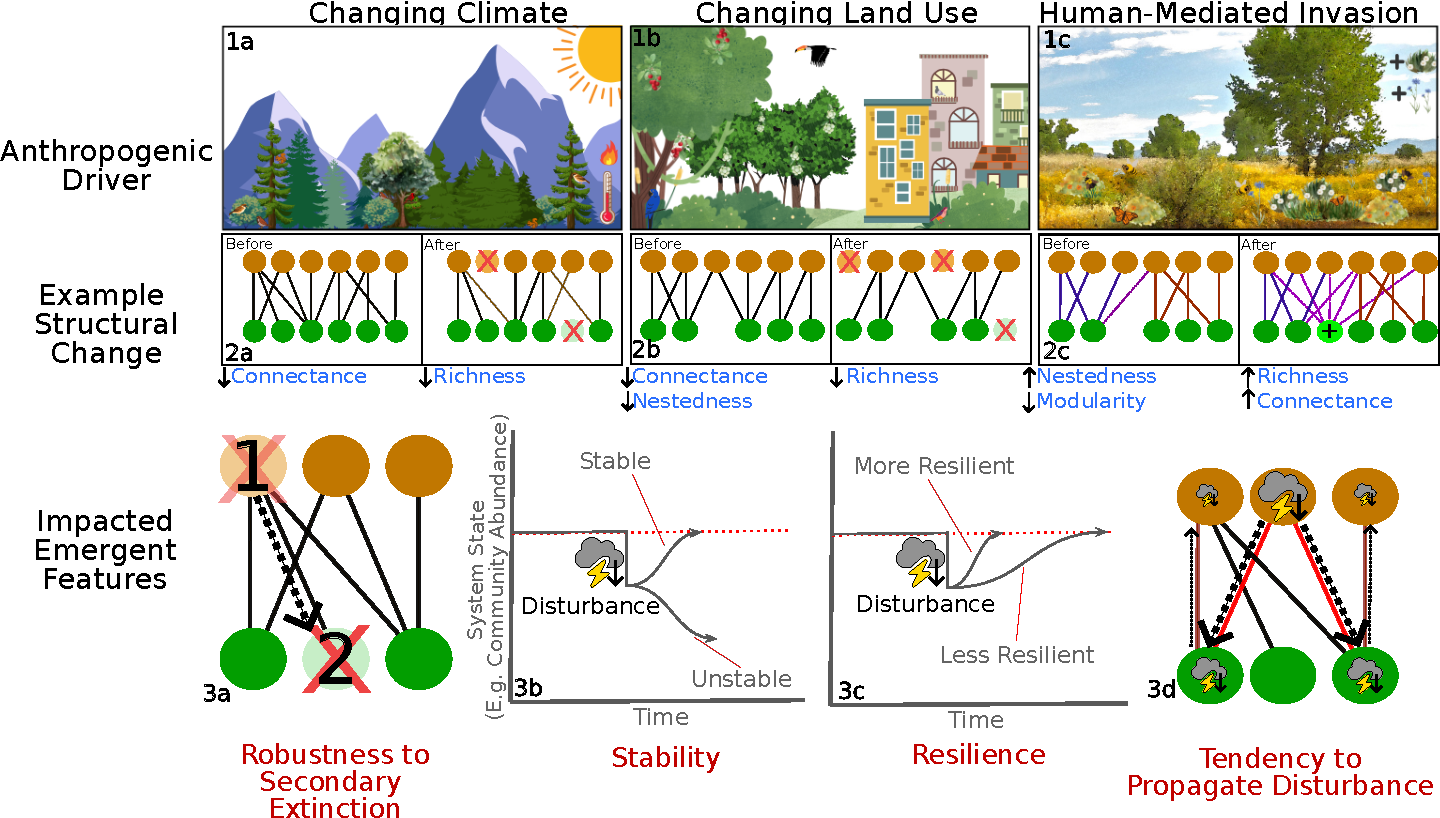
\includegraphics[width=\textwidth, alt={Graphic illustrating anthropogenic drivers of structural changes in animal-plant transport networks. The top row visualizes three main drivers, changing climate, changing land use, and human-mediated invasion, while visualizing potential network impacts. The graphic also visualized potentially impacted emergent properties of networks, including robustness to secondary extinction, stability, resilience, and tendency to propagate disturbance.}]{Review/Figures/ReviewConcept.pdf}
    \label{fig:ConceptDraft}
    \caption[Structural changes in mutualistic networks under global anthropogenic pressure]{Across a diverse set of mutualistic systems, anthropogenic drivers including changes in climate (1a), land-use patterns (1b), and the human-mediated introduction of novel mutualists (1c) can alter the structural properties of the mutualistic networks they impact (2a–2c).  These changes to component structural features may, in turn, impact emergent properties of ecological relevance (3a–3d). For example, robustness (3a) characterizes a network’s ability to avoid secondary extinctions through functional redundancy. Other emergent features describe the behavior of systems near equilibrium, including their stability—the tendency to return to equilibrium after disturbance (3b), and resilience—the speed at which they return (3c). Other features include the tendency of networks to propagate or buffer the indirect effects of disturbance (3d, where a large disturbance in the top central node's population is propagated within the network through shared links). By improving our understanding of how anthropogenic forcing elicits structural change in mutualistic networks, and how those changes translate into altered emergent properties, we can better predict and conserve mutualistic systems.}
  \end{center}
\end{figure}




